\chapter{Media Item Ranking}
\label{sec:media-item-ranking}

% the code below specifies where the figures are stored
\ifpdf
    \graphicspath{{7_media_item_ranking/figures/PNG/}{7_media_item_ranking/figures/PDF/}{7_media_item_ranking/figures/}}
\else
    \graphicspath{{7_media_item_ranking/figures/EPS/}{7_media_item_ranking/figures/}}
\fi

\section{Introduction}

In the previous chapter, we have motivated and shown methods
to deduplicate exact duplicate and near-duplicate media items.
In this chapter, we introduce ranking criteria and methods
to put deduplicated media clusters in a~well-defined order.
The application screenshots that can be seen in \autoref{fig:topvsfashionshow}
and \autoref{fig:topgrammy} show the---besides publication time (or recency)---%
most intuitive ranking criterion one can imagine:
ranking by occurrence popularity.
The more often a~media item (or a~near-duplicate of it)
appears in any of the considered social networks, 
the higher it should be ranked.
However, ranking by occurrence popularity (or media item cluster size)
disregards one of the most valuable features of social networks: 
the social aspects.
In consequence, in this chapter, we will introduce
further media item ranking criteria that,
together with media item cluster size,
will allow us to come up with more adequate social media item ranking mechanisms.

\section{Evaluating Subjective Data}

Evaluating subjective data, like \emph{the} correct ranking
for a~set of media items, is a~challenging task.
For different users, there may be different optimal settings.
A~common subjective evaluation technique
is the Mean~Opinion Score (MOS)~\cite{itu1998mos}.
Traditionally, MOS is used for conducting subjective evaluations
of telephony network transmission quality,
however, more recently, MOS has also found
wider usage in the multimedia community
for evaluating \emph{per se} subjective things
like perceived quality from the users' perspective. 
Therefore, a~set of standard, subjective tests are conducted,
where a~number of users rate the quality of test samples
with scores ranging from 1 (worst) to 5 (best).
The actual MOS is then the arithmetic mean of all individual scores.
Given a~subjective evaluation criterion
like the correctness of a~ranking,
MOS provides a~meaningful way to judge the overall quality of our approach.

\section{Media Item Ranking Criteria}

In this section, we describe several criteria that can serve to rank
media items retrieved from social networks. 
We base these criteria on the information available from
the media item extractors described in \autoref{cha:media-item-extraction},
which given event-related search terms
extract raw binary media items and associated microposts
from multiple social networks.

\subsection{Visual Ranking Criteria} \label{sec:visualrankingcriteria}

This category regards the contents of photos and videos.
We distinguish \emph{low-} and \emph{high-level} visual ranking criteria.
High-level criteria are, \emph{e.g.}, logo detection,
face recognition, and camera shot separation.
Low-level criteria are, \emph{e.g.}, file size, resolution,
duration of a~video, geolocation, and time.
Via OCR, contained characters can be treated as a~textual features.

\subsection{Audial Ranking Criteria}

This category regards the audio track of videos.
\emph{High-level} ranking criteria are the presence or absence
of silence, music, speech, or a~mixture thereof.
Similar to visual features before,
audial \emph{low-level} features are the average bit rate,
volume, possibly distorted areas, \emph{etc}.
Through audio-transcription, speech can be treated as a~textual feature.

\subsection{Textual Ranking Criteria}

This category regards the microposts that accompany media items.
Typically, microposts provide a~description of media items.
Using named-entity disambiguation tools,
textual content can be linked to LOD cloud concepts~\cite{Facebook2011}.
We have described micropost annotation in detail in \autoref{cha:micropost-annotation}.

\subsection{Social Ranking Criteria}

This category regards social network effects like shares, mentions,
view counts, expressions of (dis)likes, user diversity, \emph{etc}.
Prior work~\cite{khrouf2012aggregatingsocialmedia}
allows us to not only examine these effects
on a~\emph{single} social network,
but in a~\emph{network-agnostic} way across multiple social networks.
We will detail social aspects more later on in this chapter.

\subsection{Aesthetic Ranking Criteria}

This category regards the desired outcome after the ranking, \emph{i.e.},
the media gallery that illustrates a~given event and its atmosphere.
Studies exist for the aesthetics of
automatic photo book layout~\cite{sandhaus2011photobook},
photo aesthetics \emph{per se}~\cite{obrador2012photoaesthetics},
video and music playlist generation~\cite{knees2006musicplaylist,davidson2010videorecommendation},
however, to the best of our knowledge,
no media gallery composition aesthetics studies exist
that examine mixing video \emph{and} photo media items.

\subsection{Temporal Ranking Criteria}

This category regards the publication date of media items.
If media items are clustered, we use the youngest media item
as cluster representative.
Media items can be ranked by recency, as oftentimes more recent items
are more interesting in the streaming context of social networks.

\section{Social Interactions Abstraction Layer}
\label{sec:social-interactions-abstraction-layer}

As we have described in \autoref{cha:social-networks},
social networks have different paradigms of social interactions.
In \autoref{sec:data-format}, we have briefly presented the overall
abstraction layer on top of the native data formats
of all considered social networks in order to gain
an agnostic view on the underlying social networks.
In this section, we detail the part of the abstraction layer
that models the network-specific social interaction patterns.
Those interaction patterns must be exposed by the social network 
via specific API calls in order to be considered,
which only is the case for a~subset of the social networks we deal with.
In the subsections below, we have listed
how we abstract the social interactions in question on each social network.
In our concrete implementation, we differ unknown values
that are returned as \texttt{null}, \emph{i.e.},
where the information is not exposed,
from \texttt{0} values, where the value is known to be zero.
We briefly recall the social interactions part
of the abstraction layer's data format:

\begin{description}
  \item[\texttt{socialInteractions}] Container for social
    interactions
  \begin{description}  
  \item[\texttt{likes}] Number of times a~micropost was liked, or
    \texttt{null}
  \item[\texttt{shares}] Number of times a~micropost was shared, or
    \texttt{null}
  \item[\texttt{comments}] Number of comments a~micropost
    received, or \texttt{null}
  \item[\texttt{views}] Number of views a~micropost reached, or
    \texttt{null}
  \end{description}    
\end{description}

\subsection{Social Interaction ``Likes''}

We abstract the social interaction of liking a~media item
as instances of the following network-specific social interactions:

\begin{small_itemize}
  \item[] Facebook Like
  \item[] \googleplus \plusone
  \item[] Instagram Like
  \item[] Flickr Favorite
  \item[] YouTube Like, YouTube Favorite
  \item[] Twitter Favorite
\end{small_itemize}  

\subsection{Social Interaction ``Shares''}

We abstract the social interaction of resharing a~media item
as instances of the following network-specific social interactions:

\begin{small_itemize}
  \item[] Facebook Share
  \item[] \googleplus Share
  \item[] Twitter native ReTweet
\end{small_itemize}

\subsection{Social Interaction ``Comments''}

We abstract the social interaction of commenting on a~media item
as instances of the following network-specific social interactions:

\begin{small_itemize}
  \item[] Facebook Comments
  \item[] \googleplus Comments
  \item[] Instagram Comments
  \item[] Twitter manual, non-native ReTweet, @Replies
  \item[] Twitpic Comments
  \item[] MobyPicture Comments
  \item[] Flickr Comments
\end{small_itemize}

\subsection{Social Interaction ``Views''}

We abstract the social interaction of viewing a~media item
as instances of the following network-specific social interactions:

\begin{small_itemize}
  \item[] YouTube Views
  \item[] Flickr Views
  \item[] Twitpic Views
  \item[] Mobypicture Views
\end{small_itemize}

\section{Merging Social Interactions}
\label{sec:merging-social-interactions}

If a~set of media items is similar enough to be clustered
under the criteria that were detailed in
\autoref{cha:media-item-deduplication},
we can treat the whole of the cluster
as if it were just one media item.
Therefore, we need to specify a~merging strategy
for the associated data of the individual media items
in the particular cluster.
\autoref{code:merging} shows the pseudocode of the merging algorithm.
During the merging step,
we treat unknown values represented as \texttt{null} as \texttt{0}.
The algorithm accumulates individual social interactions
and assigns the accumulated social interactions to the cluster.

\begin{lstlisting}[caption=Pseudocode of the social interactions merging algorithm,
  label=code:merging, float]
for cluster in clusters
  likes = shares = views = comments = 0
  for mediaItem in cluster
    likes += mediaItem.likes ? mediaItem.likes : 0
    shares += mediaItem.shares ? mediaItem.shares : 0
    comments += mediaItem.comments ? mediaItem.comments : 0
    views += mediaItem.views ? mediaItem.views : 0
  end for
  cluster.socialInteractions.likes = likes
  cluster.socialInteractions.shares = shares
  cluster.socialInteractions.comments = comments
  cluster.socialInteractions.views = views
end for     
\end{lstlisting}

\section{Selection of a~Cluster's Visual Representative}  

As outlined in the previous section, similar enough media items
are clustered and treated as just one media item.
The previous section introduced
a~merging algorithm for the social interactions data.
In this section, we introduce an algorithm for the selection of
a~cluster's visual representative.
Naturally, through the way the clustering algorithm works,
the contained media items are already visually similar. 
In consequence, we fall back to using \emph{low-level}
visual ranking criteria as defined in \autoref{sec:visualrankingcriteria}.
\autoref{code:clusterrepresentative} shows the cluster representative
selection algorithm, which is based on the low-level feature \emph{resolution}.
The algorithm selects the media item with the highest megapixel resolution
as the cluster representative.

\begin{lstlisting}[caption=Pseudocode of the cluster representative selection algorithm,
  label=code:clusterrepresentative, float]
maxPixels = 0
clusterRepresentative = null
for mediaItem in cluster
  resolution = mediaItem.width * mediaItem.height
  if resolution >= maxPixels
    maxPixels = resolution
    clusterRepresentative = mediaItem
  end if  
end for
return clusterRepresentative     
\end{lstlisting}

\section{Ranking Media Item Clusters}

Up to now, we have shown how media item clusters are formed,
how each cluster's social interactions social interactions data is accumulated,
and how a~cluster's representative media item is selected.
In this section, we finally describe a~ranking formula to rank
a~set of media clusters that match a~given query.

In the ranking formula, we consider all the previously defined ranking criteria,
namely these are visual, audial, textual, temporal, social, and aesthetic.
For a~given set of media item clusters, a~ranking is calculated as follows.
$$ \alpha \times \mathit{likes} + \beta \times \mathit{shares} +
\gamma \times \mathit{comments} + \delta \times \mathit{views} +
\epsilon \times \mathit{crossNetwork} + \zeta \times \mathit{recency} $$
With the weight factors
$$ \alpha, \beta, \gamma, \delta, \epsilon, \zeta \in \mathbb{N} $$
The values $ \mathit{likes}, \mathit{shares}, \mathit{comments}, \mathit{views} $
stem from the individual media items as defined in \autoref{sec:data-format} and 
were accumulated as defined in \autoref{sec:merging-social-interactions}.
The value of $ \mathit{crossNetwork} $ corresponds to the length of the current cluster. 
Finally, the value of $ \mathit{recency} $ is calculated as follows.
If the youngest media item in the cluster is less than or exactly one day old, the value of
$ mathit{recency} $ is 8, for two days it is 4, for three days it is 2, and for each day more, the value is 1.

\section{Evaluation}

\subsection{Super Bowl Analyses by Social Networks}

We have evaluated our approach with the at time of writing
recent event of the Super Bowl XLVII%
\footnote{\url{http://en.wikipedia.org/wiki/Super_Bowl_XLVII},
accessed February 8, 2013}.
This event received broad social media coverage, and the social networks
Twitter\footnote{\url{http://blog.twitter.com/2013/02/the-super-tweets-of-sb47.html},
accessed February 8, 2013},
Instagram\footnote{\url{http://blog.instagram.com/post/42254883677/sbroundup},
accessed February 8, 2013}, and
Facebook\footnote{\url{http://newsroom.fb.com/News/570/Super-Bowl-XLVII-on-Facebook},
accessed February 8, 2013} all published blog posts with analyses of the event
on the respective networks,
whereas the search engine Google%
\footnote{\url{http://googleblog.blogspot.com/2013/02/m-beyonce-and-ravens-dominate-game-day.html},
accessed February 8, 2013}
published an analysis of trending queries during the match.
In the following, we provide summaries of these different analyses,
with the expectation to encounter relevant media items
for each of the mentioned highlights in the final ranked list of media items
stemming from the various social networks.

According to Twitter's analysis, the five moments that generated the most tweets
during the game (see the Wikipedia-provided game summary for details)
ordered by decreasing number of tweets per minute were
the power outage,
the 108-yard kickoff return for the Ravens touchdown by Jones,
the moment when the clock expired and the Ravens won,
Jones catches a~56 yard pass for a~Ravens touchdown,
and the Gore touchdown for the 49ers.
Overall, 24.1 million tweets about the game and halftime show were counted,
a~number that even leaves aside the advertisements.
The Twitter article further mentions the performance by superstar artist Beyoncé 
and a~number of Super Bowl advertisements as highlights of the event.   

Instagram's analysis mentions that more than three million photos
with Super Bowl-related words in their captions were shared and
at peak more than 450 photos about the game were posted every second.
During the halftime show, over 200 photos per second were posted about Beyoncé.
The blog post further highlights how a~TV channel pointed to selected photos
and explains that brands ran Instagram campaigns.
According to Instagram, people used Instagram both directly at the event venue,
but also while watching from home.

Facebook's analysis mentions as top five most talked-about moments of the Super Bowl 
the moment when the Ravens win the Super Bowl, 
Beyoncé's halftime performance,
the blackout in the Superdome,
Jacoby Jones' 108-yard kickoff return for a Ravens touchdown, and
Joe Flacco’s 56-yard pass to Jacoby Jones for a Ravens touchdown.
The Super Bowl was nicknamed the Harbaugh Bowl, as both teams' head coaches
are named Harbaugh as last name.
Facebook also mentions Alicia Keys' performance of the National Anthem as special event.

The search engine Google has compiled a~list of top trending search terms
during the match, with the top ones being M\&M's, Beyoncé, Baltimore Ravens,
San Francisco 49ers, and Colin Kaepernick (quarterback for the San Francisco 49ers).
Additional spiking search terms were power outage
and Chrysler (driven by an advertisement during the game).
Further advertisement-related search terms were for advertisements for M\&M's,
Mercedes-Benz, Disney’s Oz Great and Powerful movie, Lincoln, and Audi.

While no separate statistics are available yet at time of writing
for the video hosting platform YouTube,
Google's blog post mentions that searches for Gangnam Style were trending on YouTube,
along with searches for big game performers Alicia Keys and Beyoncé.

\subsection{Expected Super Bowl Media Items}

Given the previous social network analyses, we expect to see media items
on the following topics (in no particular order):

\begin{small_itemize}
  \item[] the power outage
  \item[] the performances of Beyoncé and Alicia Keys
  \item[] the advertisements
  \item[] the match itself
  \item[] the Super Bowl watchers  
\end{small_itemize}

\autoref{fig:loose_order} and \autoref{fig:strict_order} show media items
for the two queries 49ers and Baltimore Ravens arranged
in two different media gallery styles, loose order and strict order.
For details on media gallery generation, we refer the reader to the upcoming
\autoref{cha:media-item-compilation}.

\begin{figure}[htb]
  \centering
  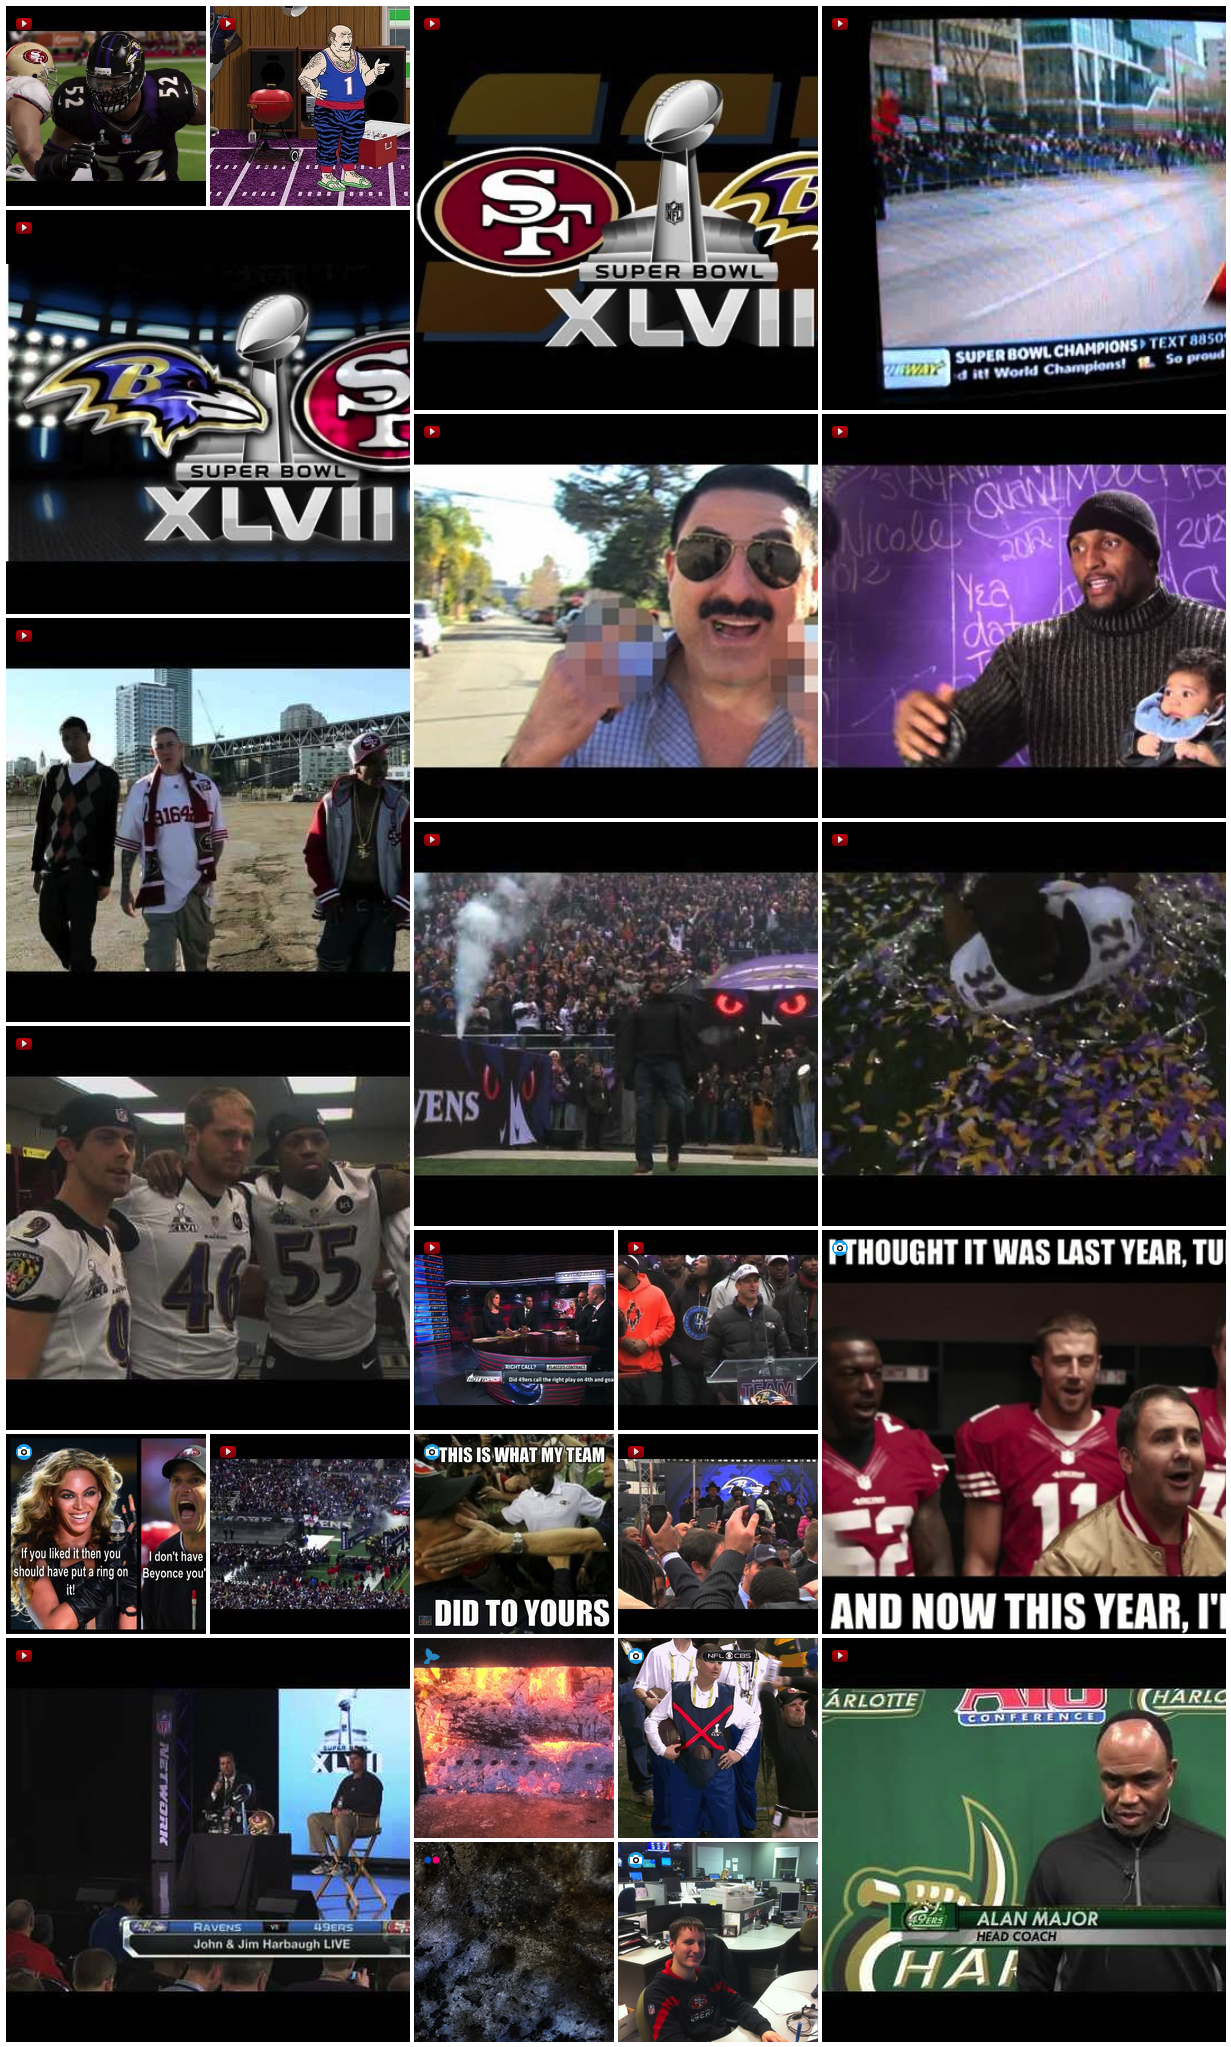
\includegraphics[width=0.75\linewidth]{loose_order.png}
  \caption[Ranked Super Bowl media gallery in loose order]
  {Ranked Super Bowl media gallery in loose order}
  \label{fig:loose_order}
\end{figure}

\begin{sidewaysfigure}
  \centering
  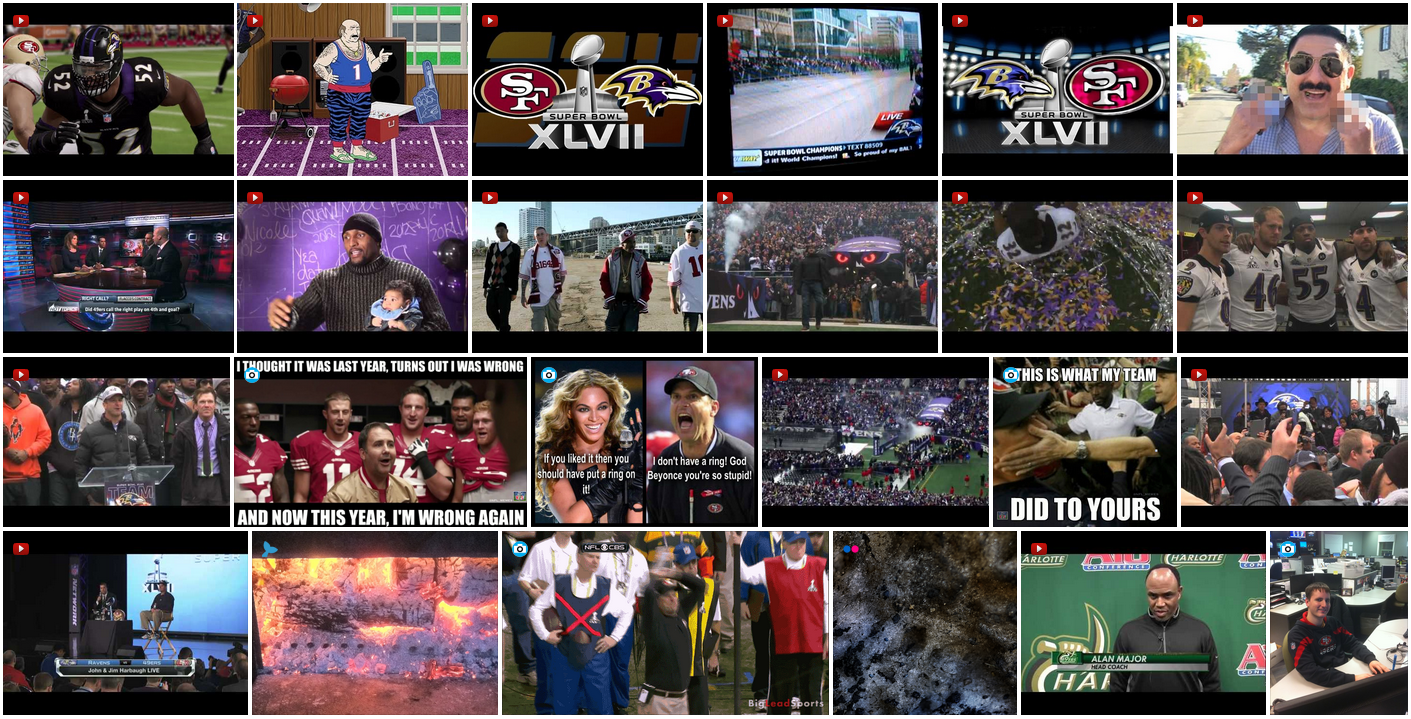
\includegraphics[width=0.75\linewidth]{strict_order.png}
  \caption[Ranked Super Bowl media gallery in strict order]
  {Ranked Super Bowl media gallery in strict order \todo{Check final orientation}}
  \label{fig:strict_order}
\end{sidewaysfigure}  


\section{Conclusion}

\section*{Chapter Notes}
This chapter is partly based on the following publications:
\todo{Add publications}